\begin{figure}[H]
\centering
\includegraphics[page=6,width=0.48\textwidth]{\FCNCFigures/xTFW/raw/NOMINAL/reg2mtau1b2jos_vetobtagwp70_highmet/tau_pt_0.pdf}
\put(-100, 140){\textbf{(a1)}}
\put(-120, 130){\footnotesize{$t_h\thadhad$-2j (OS)}}
\includegraphics[page=6,width=0.48\textwidth]{\FCNCFigures/xTFW/raw/NOMINAL/reg2mtau1b3jos_vetobtagwp70_highmet/tau_pt_0.pdf}
\put(-100, 140){\textbf{(b1)}}
\put(-120, 130){\footnotesize{$t_h\thadhad$-3j (OS)}}\\
\includegraphics[page=6,width=0.48\textwidth]{\FCNCFigures/xTFW/raw/NOMINAL/reg2mtau1b2jss_vetobtagwp70_highmet/tau_pt_0.pdf}
\put(-100, 140){\textbf{(a2)}}
\put(-120, 130){\footnotesize{$t_h\thadhad$-2j (SS)}}
\includegraphics[page=6,width=0.48\textwidth]{\FCNCFigures/xTFW/raw/NOMINAL/reg2mtau1b3jss_vetobtagwp70_highmet/tau_pt_0.pdf}
\put(-100, 140){\textbf{(b2)}}
\put(-120, 130){\footnotesize{$t_h\thadhad$-3j (SS)}}
\caption{ The distributions of leading $\tau$ $\pt$ in the $t_h\thadhad$-2j (a1), and $t_h\thadhad$-3j (b1)  Signal Regions. Comparison of the $\tau$ $\pt$ distributions for the background and data in the $t_h\thadhad$-2j (a2), and $t_h\thadhad$-3j (b2) Same Sign Control Regions before the fake estimation. Data is more than the MC prediction because the fake tau backgrounds are not yet added, which will be estimated using Fake Factor Method. The lower pads in CRs (a2,b2) are empty since the overshooting of data against the MC prediction. Only statistical uncertainties are being shown. Underflow and overflow bins are included respectively in the first and last bins.}
\label{fig:os_pre_hadhad}
\end{figure}
